\documentclass[../../main.tex]{subfiles}


\begin{document}
    The NA62 experiment is a fixed target experiment located in the north area of CERN. It aims to measure the branching fraction of the ultra-rare charged kaon decay $K^+ \rightarrow \pi^+ \nu \bar{\nu}$ to a 10\% precision, similar to theoretical SM calculations shown in the previous section. A target of 100 events has been set to obtain this precision, requiring the exposure of kaon decays in the order of $10^{13}$. 
    \newline The experiment employs a decay-in-flight technique to obtain a large number of charged kaon decays within the short time frame of a few years. The beam used in NA62 is produced from a 400\,GeV proton beam from the Super Proton Synchrotron (SPS) incident on a Beryllium target (T10), resulting in a secondary beam containing charged kaons. The secondary beam produced has a momentum of 75\,GeV and has a composition of mostly pions (70\,\%), protons (23\,\%), kaons (6\,\%) and a small number of muons ($<$1\,\%). 
    \subsection{Detector Setup}\label{seq:1}
    The NA62 detector comprises several sub-detectors. This subsection will cover a basic overview of the sub-detectors, with more in-depth explanations for sub-detector relevant to the symmetric setup. 
    \begin{figure}[H]
        \centering
        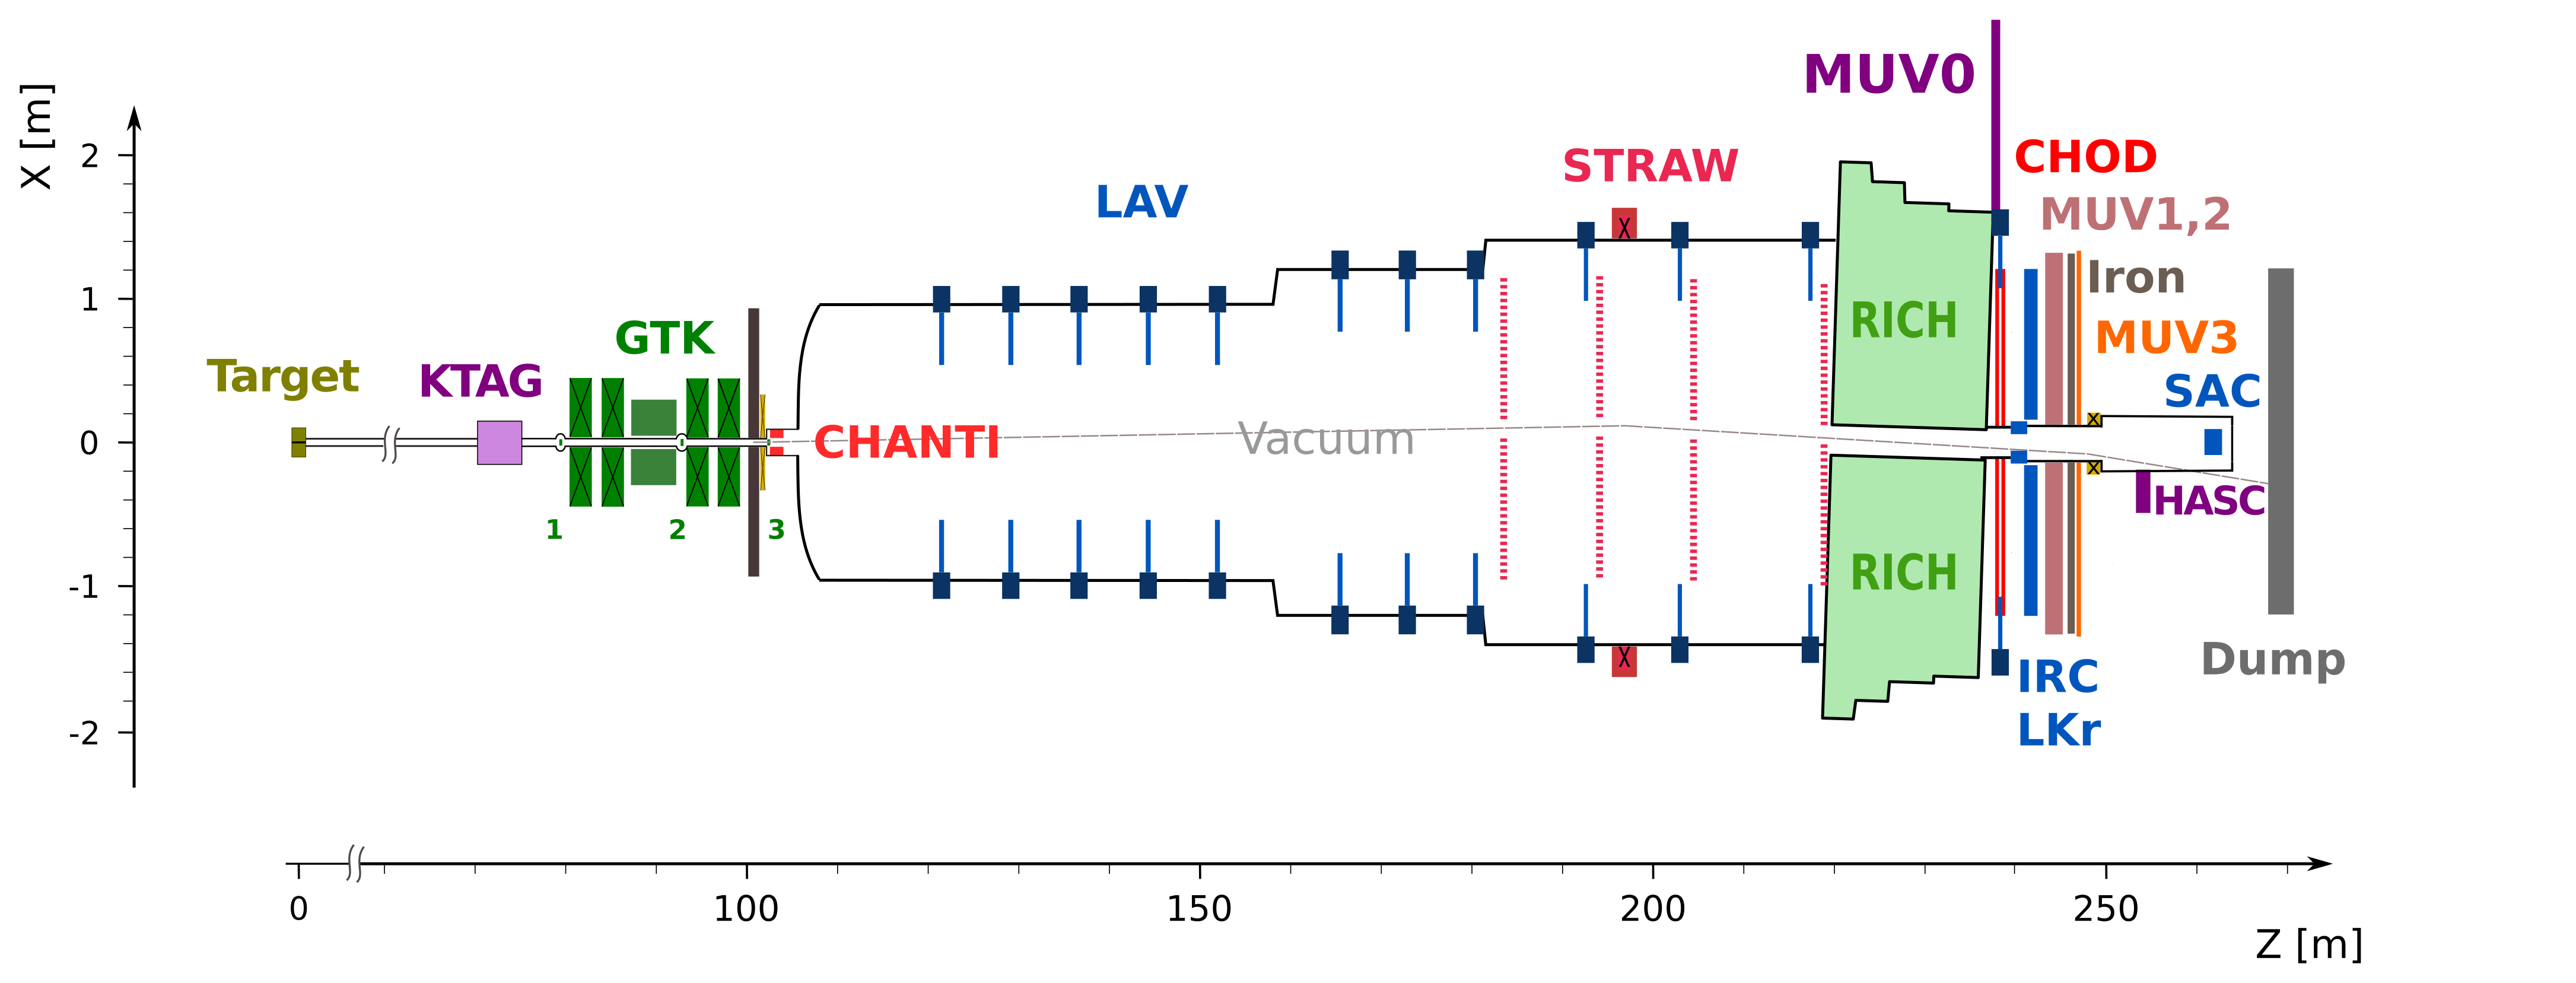
\includegraphics[width=13cm]{imgs/na62DetDia.png}
        \caption{X-Z diagram of NA62 detector setup for Run 1}
        \label{fig:na62-det}
    \end{figure}
    \noindent From the T10 target, the charged kaon beam travels through the beam pipe to the experimental hall ECN3, where the first sub-detector is found. A differential Cherenkov detector tags the charged kaons in the beam. Cherenkov light is produced by charged particles passing through a CERN CEDAR vessel filled with Nitrogen gas at a pressure of around 1.75\,bar \cite{Bovet:1982xf}. 
    Due to the high intensity and tight time resolution requirements employed at NA62, the original photo-detectors (PMT's) and front-end electronics were inadequate. The KTAG has been developed for the NA62 to meet the high kaon rate requirements and time resolution requirements of $\mathcal{O}(100ps)$.
    \newline Downstream of the KTAG is the beam spectrometer named the Giga Tracker (GTK). The GTK comprises 4 silicon trackers stations to measure the beam's position, time and momentum. As the GTK is directly in the beamline, vetoing any particles produced from inelastic interactions is essential. This is done by the Charged Anti-coincidence detector (CHANTI) located slightly downstream of the final GTK station. The CHANTI detects charged particles using polystyrene base scintillators.
    \newline The main decay volume is located downstream of the CHANTI and is in a large vacuum tube shown in figure \ref{fig:na62-det}. This is where kaons are allowed to decay if they are to be within the acceptance of the various sub-detectors. Downstream from this is the STRAW Spectrometer which provides kinematic measurements of the charged products of the kaon decays. It consists of four spectrometer chambers and a dipole magnet (MNP33) with two of the chambers located before the magnet and two after. A more detailed description of this detector is provided in section \ref{STRAW}.
    \newline The Ring Imaging Cherenkov (RICH) follows the last straw chamber and is a 17\,m long neon-filled vessel. It is designed to distinguish between pions and muons and is part of the Particle Identification system (PID). This is also complemented by the Muon Veto (MUV) system comprising two hadronic calorimeters (MUV1 and MUV2)
    \newline A Photon-Veto system provides coverage of photons produced from the decay region up to 50\,mrad with respect to the z-axis. This includes:
    \begin{itemize}
        \item 12 Large Angle Vetos (LAVs) placed along the decay region, between STRAW spectrometer chambers and after the RICH. Providing coverage of photons emitted at angles from 8.5 to 50\,mrad \cite{Gil_2017}.
        \item Liquid Krypton calorimeter (LKr) which is located after the RICH and was used in the predecessor experiment NA48. 
        \item Small Angle Veto (SAV) system, comprising of two shashlyk calorimeters named the Small Angle Calorimeter (SAC) and the Intermediate-Ring Calorimeter (IRC) which provides photon veto coverage for  small angles.
    \end{itemize}
    There are several other detectors, such as the MUV3, which provides fast signals for use in the L0 trigger system and a pair of Charged Particle Hodoscopes (CHODs), which also provide input to the L0 trigger system. Some additional veto detectors, such as MUV0 and the HASC are used to for analysis. 
    \newline For the new run (after LS2), there have been several additions to the detector setup. The ANTI-0 detector is a hodoscope placed downstream of the CHANTI before the decay volume, used to veto halo particles (mostly muons) that enter the decay volume \cite{Danielsson:2723429}.
     A second detector system has been implemented between the GTK stations to veto any decay products of kaons decaying between the GTK stations, named the Veto Counter (VC), it is made up of three stations of scintillators between GTK stations 3 and 2.
    \newline Two sub-detectors, KTAG and STRAW spectrometer, will be described in more detail due to their relevance to the studies that are planned for my PhD. The KTAG-CEDAR has been selected due to my involvement in the CEDAR-H test beam. The STRAW spectrometer has been selected due to my participation in the development of flexibility of the sub-detector and its subsequent use in the symmetric NA62 study later on in this report.
    \subsubsection{KTAG}\label{CEDAAR}
    As mentioned previously, kaons are identified in the beam by the CEDAR-KTAG subdetector. The charged beam produces  Cherenkov light when passing through the Nitrogen gas-filled CEDAR. The light produced is then reflected onto a ring-shaped diaphragm by the Mangin mirror, located at the end of the CEDAR vessel, which is a special geometry to produce the ring shape needed to distinguish particles. Between the mirror and the diaphragm, the light passes through a chromatic corrector lens that corrects for the dispersion caused by the gas. The diaphragm only allows the light of a certain radius to pass through, allowing the selection of certain particles corresponding light. The particle is selected by altering the pressure of the gas. After the diaphragm the light passes through several quartz windows into the KTAG enclosure. 
    \begin{figure}[H]
        \centering
        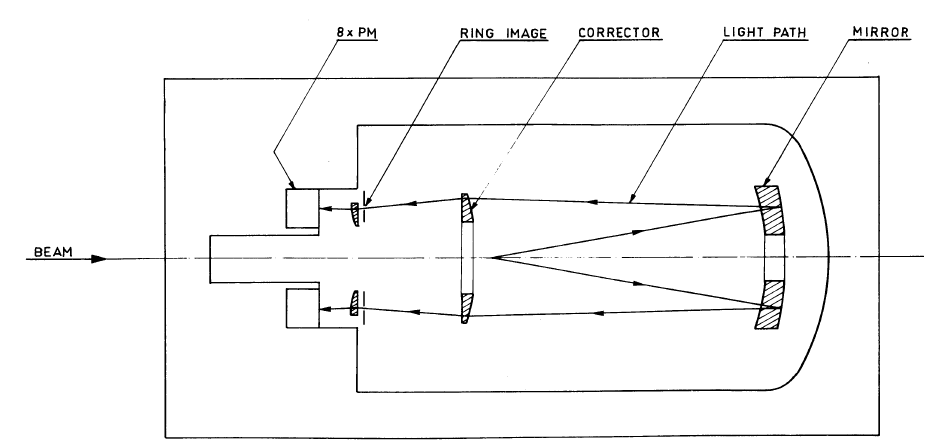
\includegraphics[width=10cm]{imgs/CedarOldDia.png}
        \caption{Diagram describing the CEDAR optics \cite{Bovet:1982xf}}
        \label{fig:Cedar_dia}
    \end{figure}
    \noindent The light is reflected by eight spherical mirrors located around the beam pipe into eight light boxes, which are seen in figure \ref{fig:Ktag}. Each lightbox (commonly referred to as sectors) contains 48 photomultipliers converting the light into electrical signals that are then collected by the front-end electronics. 
    \newline At the start of a data-taking period, a pressure scan is completed to isolate the kaon peak from the other constituents of the beam. Through tests and pressure scans, the optimal pressure for kaons is set at 1.75\,bar. Considering the quartz windows and the Nitrogen gas, the total material path of the beam is $3.5 \times 10^{-2} X_0$ \cite{Gil_2017}.
    \begin{figure}[H]
        \centering
        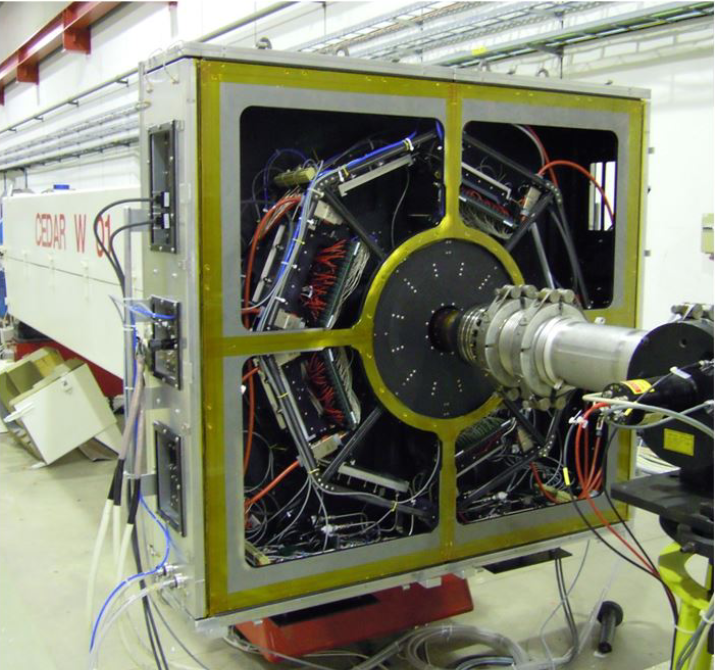
\includegraphics[width=7cm]{imgs/KtagOpenPic.png}
        \caption{Photo of CEDAR and KTAG installed in the NA62 beamline}
        \label{fig:Ktag}
    \end{figure}
    \noindent Improving the material budget is possible by replacing Nitrogen with Hydrogen at a higher pressure of 3.9\,bar, resulting in a reduced material path of $7 \times 10^{-3} X_0$. 
    \subsubsection{STRAW Spectrometer}\label{STRAW}
    The STRAW Spectrometer is used for kinematic measurements of charged decay products and comprises of four separate chambers and one dipole magnet (MNP33). The chambers are located downstream from the decay region, with chambers 1 and 2 separated by 10\,m with the MNP33 magnet placed downstream of chamber 2. Chambers 3 and 4 are located downstream of the MNP33 with a separation of 14\,m. Each chamber comprises four views, containing four layers of straws in a pattern shown in figure \ref{fig:strawsp}. The straws are 2.1\,m long drift tubes that are about 9.75\,mm in diameter containing an $ArCO_2$ gas mixture and are similar to proportional counters. As a particle passes through the gas, it ionises the gas producing a signal in the central wire. This allows for a measurement of the spatial position of the particle, which, along with the MNP33 allows for momentum calculations of the particles.
    \begin{figure}[H]
        \centering
        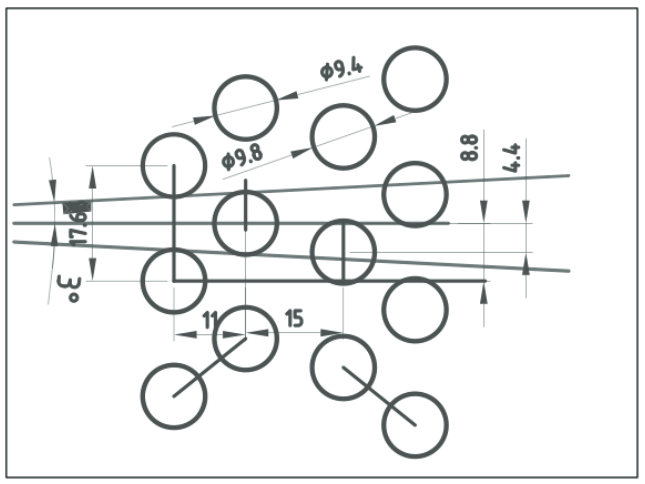
\includegraphics[width=7cm]{imgs/straw_diagram.png} 
        \caption{Diagram of straw placement in each view \cite{SERGI2012530}}
        \label{fig:strawsp}
    \end{figure}

    \ifSubfilesClassLoaded{%
        \bibliographystyle{IEEEtran}
        \bibliography{../../../references.bib}%
    }{} 
\end{document}